\documentclass[sigconf,authorversion,nonacm]{acmart}

\usepackage{minted}
\usemintedstyle{borland}
\setminted{linenos=true,fontsize=\large}

\usepackage{fontspec}
\setmonofont{Fira Code Retina}[Scale=MatchLowercase]

\captionsetup{justification=centering,margin=1cm}

\AtBeginDocument{%
  \providecommand\BibTeX{{%
    \normalfont B\kern-0.5em{\scshape i\kern-0.25em b}\kern-0.8em\TeX}}}

\begin{document}

\title{Tarea 4 \\ Algoritmos genéticos}

\author{Mario Emilio Jiménez Vizcaíno}
\email{A01173359@itesm.mx}
\affiliation{}

\author{Jesus Abraham Haros Madrid}
\email{A01252642@itesm.mx}
\affiliation{}


\maketitle

\section{Introducción}
Durante las últimas décadas, una de las grandes inspiraciones para los avances en la inteligencia artificial ha sido la naturaleza, y los algoritmos genéticos no son la excepción. Este tipo de algoritmos se basan en 3 operaciones simples sobre vectores de bits: la cruza, la mutación y la selección, para así poder imitar los mecanismos de la selección natural y la reproducción.\cite{holland1992genetic}

En esta práctica utilizamos 3 algoritmos genéticos para resolver el problema de la mochila, mejor conocido como \textit{Knapsack problem}, en el que se tiene una lista de ítems con pesos y valores, y el objetivo es seleccionar de la lista una combinación de ítems cuya suma de valores sea máxima, mientras la suma de sus pesos sea inferior a un límite predefinido.


\section{Metodología e implementación}
Para la realizar la implementación de este problema utilizamos la librería \textit{deap} de Python, la cual implementa los 3 algoritmos genéticos presentados.\cite{DEAP_JMLR2012} La implementación del algoritmo puede ser encontrada el apéndice \ref{app:py}.

\subsection{Representación de los individuos}
La generación y administración de los individuos es una tarea que la librería maneja por nosotros, aunque si especificamos cómo generar los atributos de los individuos (cada bit del vector, utilizando números aleatorios para generar un bit), cómo generar cada individuo (repitiendo la generación del atributo $n$ veces, siendo $n$ el número de ítems de los cuales podemos escoger), y cómo generar a la población (repitiendo la generación del individuo, en nuestro caso 10 veces).

Concretamente, cada uno de los individuos de la población está formado de 24 bits, inicialmente aleatorios.

\subsection{Función de evaluación}
La función de evaluación es muy simple, y está formada por dos pasos:
\begin{enumerate}
  \item El cálculo de la suma de los valores de los ítems seleccionados, primero multiplicando los bits del individuo (0/1) por la lista de valores de los ítems, y finalmente sumando los valores. Esta suma determina qué tan eficiente es el individuo, y el objetivo del algoritmo es maximizarla.
  \item El cálculo de la suma de los pesos de los ítems seleccionados, que es usado para que, en caso de que exceda el límite predefinido, la evaluación del individuo sea penalizada. En nuestro caso preferimos solamente asignarle una evaluación de 0.
\end{enumerate}

\subsection{Algoritmos genéticos}
Los tres algoritmos genéticos principales se explican a continuación.

\subsubsection{EA simple}
Este algoritmo utiliza una población de individuos, que son cruzados entre sí y sufren mutaciones aleatorias. Como consecuencia de que los individuos pueden sufrir modificaciones sin importar si tuvieron una buena evaluación o no, el algoritmo puede tener resultados muy variados.

\subsubsection{EA $(\mu + \lambda)$}
Este algoritmo y el siguiente tienen en común que sólo sufren una variación, ya sea cruce o mutación. En el caso de este algoritmo, la nueva generación se escoje de un conjunto de los hijos y su descendencia, por lo que si algún padre tiene una mejor evaluación que sus hijos, puede continuar produciendo hijos en las siguientes generaciones.

\subsubsection{EA $(\mu , \lambda)$}
Este algoritmo es muy parecido al anterior, pero difiere en que la siguiente generación de la población sólo se selecciona de la descendencia de los padres. Esto produce una mayor rapidez de "exploramiento" de posibles resultados, aunque perdiendo a los padres en cada generación.


\section{Resultados}
\subsection{Mejores instancias}
Las mejores instancias que obtuvimos durante la ejecución de los algoritmos fueron las siguientes. También incluímos un porcentaje que describe qué tan cerca estuvieron de la solución óptima de 13,549,094.

\subsubsection{EA simple}
\begin{enumerate}
  \item 13,452,724 (99.289\%)
  \item 13,375,768 (98.721\%)
  \item 13,354,550 (98.564\%)
\end{enumerate}

\subsubsection{EA $(\mu + \lambda)$}
\begin{enumerate}
  \item 13,461,886 (99.357\%)
  \item 13,433,220 (99.145\%)
  \item 13,419,377 (99.043\%)
\end{enumerate}

\subsubsection{EA $(\mu , \lambda)$}
\begin{enumerate}
  \item 13,518,963 (99.778\%)
  \item 13,396,655 (98.875\%)
  \item 13,377,418 (98.733\%)
\end{enumerate}

\subsection{Curva de mejor encontrado}
A continuación se muestran tres gráficas, una por cada algoritmo, de la mejor evaluación encontrada por cada generación, promediada entre las 10 ejecuciones de los algoritmos.

\subsubsection{EA simple}
Este algoritmo tuvo la mayor desviación estándar como consecuencia de que las variaciones se aplicaban a todos los individuos sin importar si tenían o no una buena evaluación.

\begin{figure}[H]
  \centering
  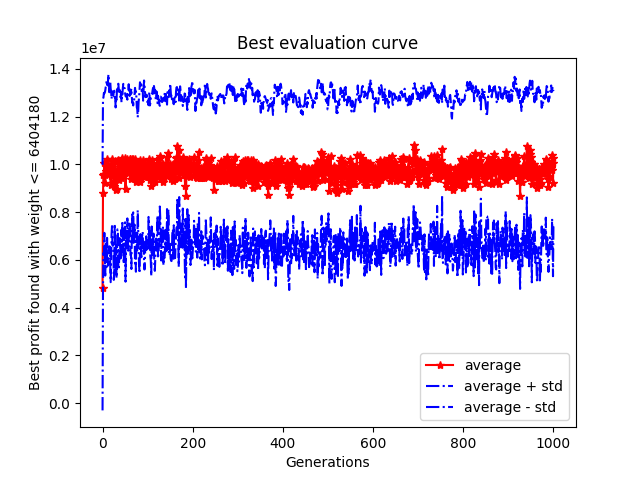
\includegraphics[width=210pt]{simple.png}
\end{figure}

\subsubsection{EA $(\mu + \lambda)$}
En la gráfica de este algoritmo se puede apreciar que los cambios y las mutaciones son mucho más suaves, ya que se le permitía a los padres formar parte de las siguientes iteraciones, y por lo tanto era más difícil hacer grandes cambios en la población general.

\begin{figure}[H]
  \centering
  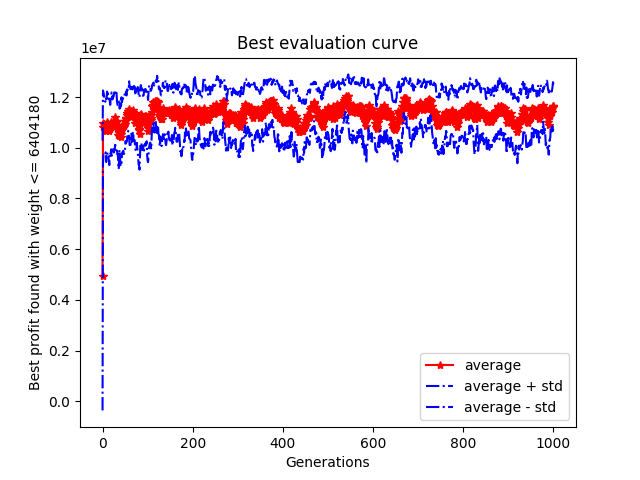
\includegraphics[width=210pt]{plus.png}
\end{figure}

\subsubsection{EA $(\mu , \lambda)$}
Finalmente esta gráfica tiene un gran parecido con la gráfica anterior, pero se puede observar cambios más rápidos y "aleatorios" ya que la descendencia a través de las generaciones podía tener evaluaciones más variadas que en el algoritmo anterior.

\begin{figure}[H]
  \centering
  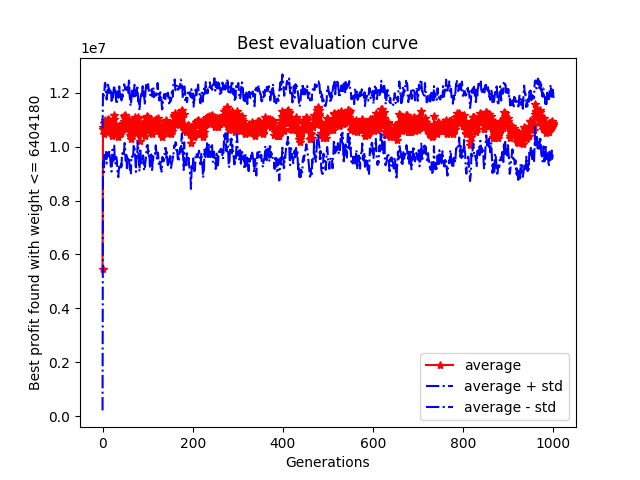
\includegraphics[width=210pt]{comma.png}
\end{figure}


\section{Conclusiones y retos encontrados}
Los algoritmos genéticos nos presentan una forma diferente y útil de resolver problemas que pueden ser representados de manera simple, aunque si creemos que la selección de parámetros iniciales y la configuración de los algoritmos es una tarea que merece una investigación exclusiva.

Los principales retos que tuvimos fueron al comprender cómo funciona la librería \textit{deap}, ya que fue de gran utilidad para describir y ejecutar los algoritmos genéticos a través de las funciones que ofrece la librería, pero también utilizando un par ejemplos proporcionados por el profesor como base.


\bibliographystyle{ACM-Reference-Format}
\bibliography{references}

\clearpage

\appendix

\begin{figure*}
  \section{Implementación de los algoritmos genéticos}
  \label{app:py}
  \inputminted[lastline=44]{python}{/home/mario/git/MarioJim/PracticasInteligenciaComp/4_AlgoritmosGeneticos/A01173359_A01252642_T4.py}
\end{figure*}

\begin{figure*}
  \inputminted[firstline=46]{python}{/home/mario/git/MarioJim/PracticasInteligenciaComp/4_AlgoritmosGeneticos/A01173359_A01252642_T4.py}
\end{figure*}

\end{document}
\endinput